
\chapter{Appendix}



\section{Somato-dendritic coupling}\label{sec-somato-dendr}

\cite{urbanczik2014learning} discuss a possible extension to their neuron- and plasticity model, in which the
dendro-somatic coupling transmits voltages in both directions. They show that the plasticity rule requires only minor
adaptations for successfull learning under this paradigm. Yet, as described by passive cable theory, the flow between
neuronal compartments is dictated by their respective membrane capacitances. These are calculated from their membrane
areas, which vastly differ in the case of pyramidal neurons. \todo{find a nice citation for }


15,006 458


will not be considered here. The motivation is, that dendritic membrane area is


\section{Presentation times and Latent Equilibrium}\label{sec-appendix-t-pres}

Exactly matching parameters and the training environment to those of existing implementations turned out to be a 
significant challenge. Particularly the way NEST handles signal transmissions made and exact numerical replication of
results impossible, as discussed in Section \todo{talk about timing differences}. In order to validate, that  



\begin{figure}
    \centering
    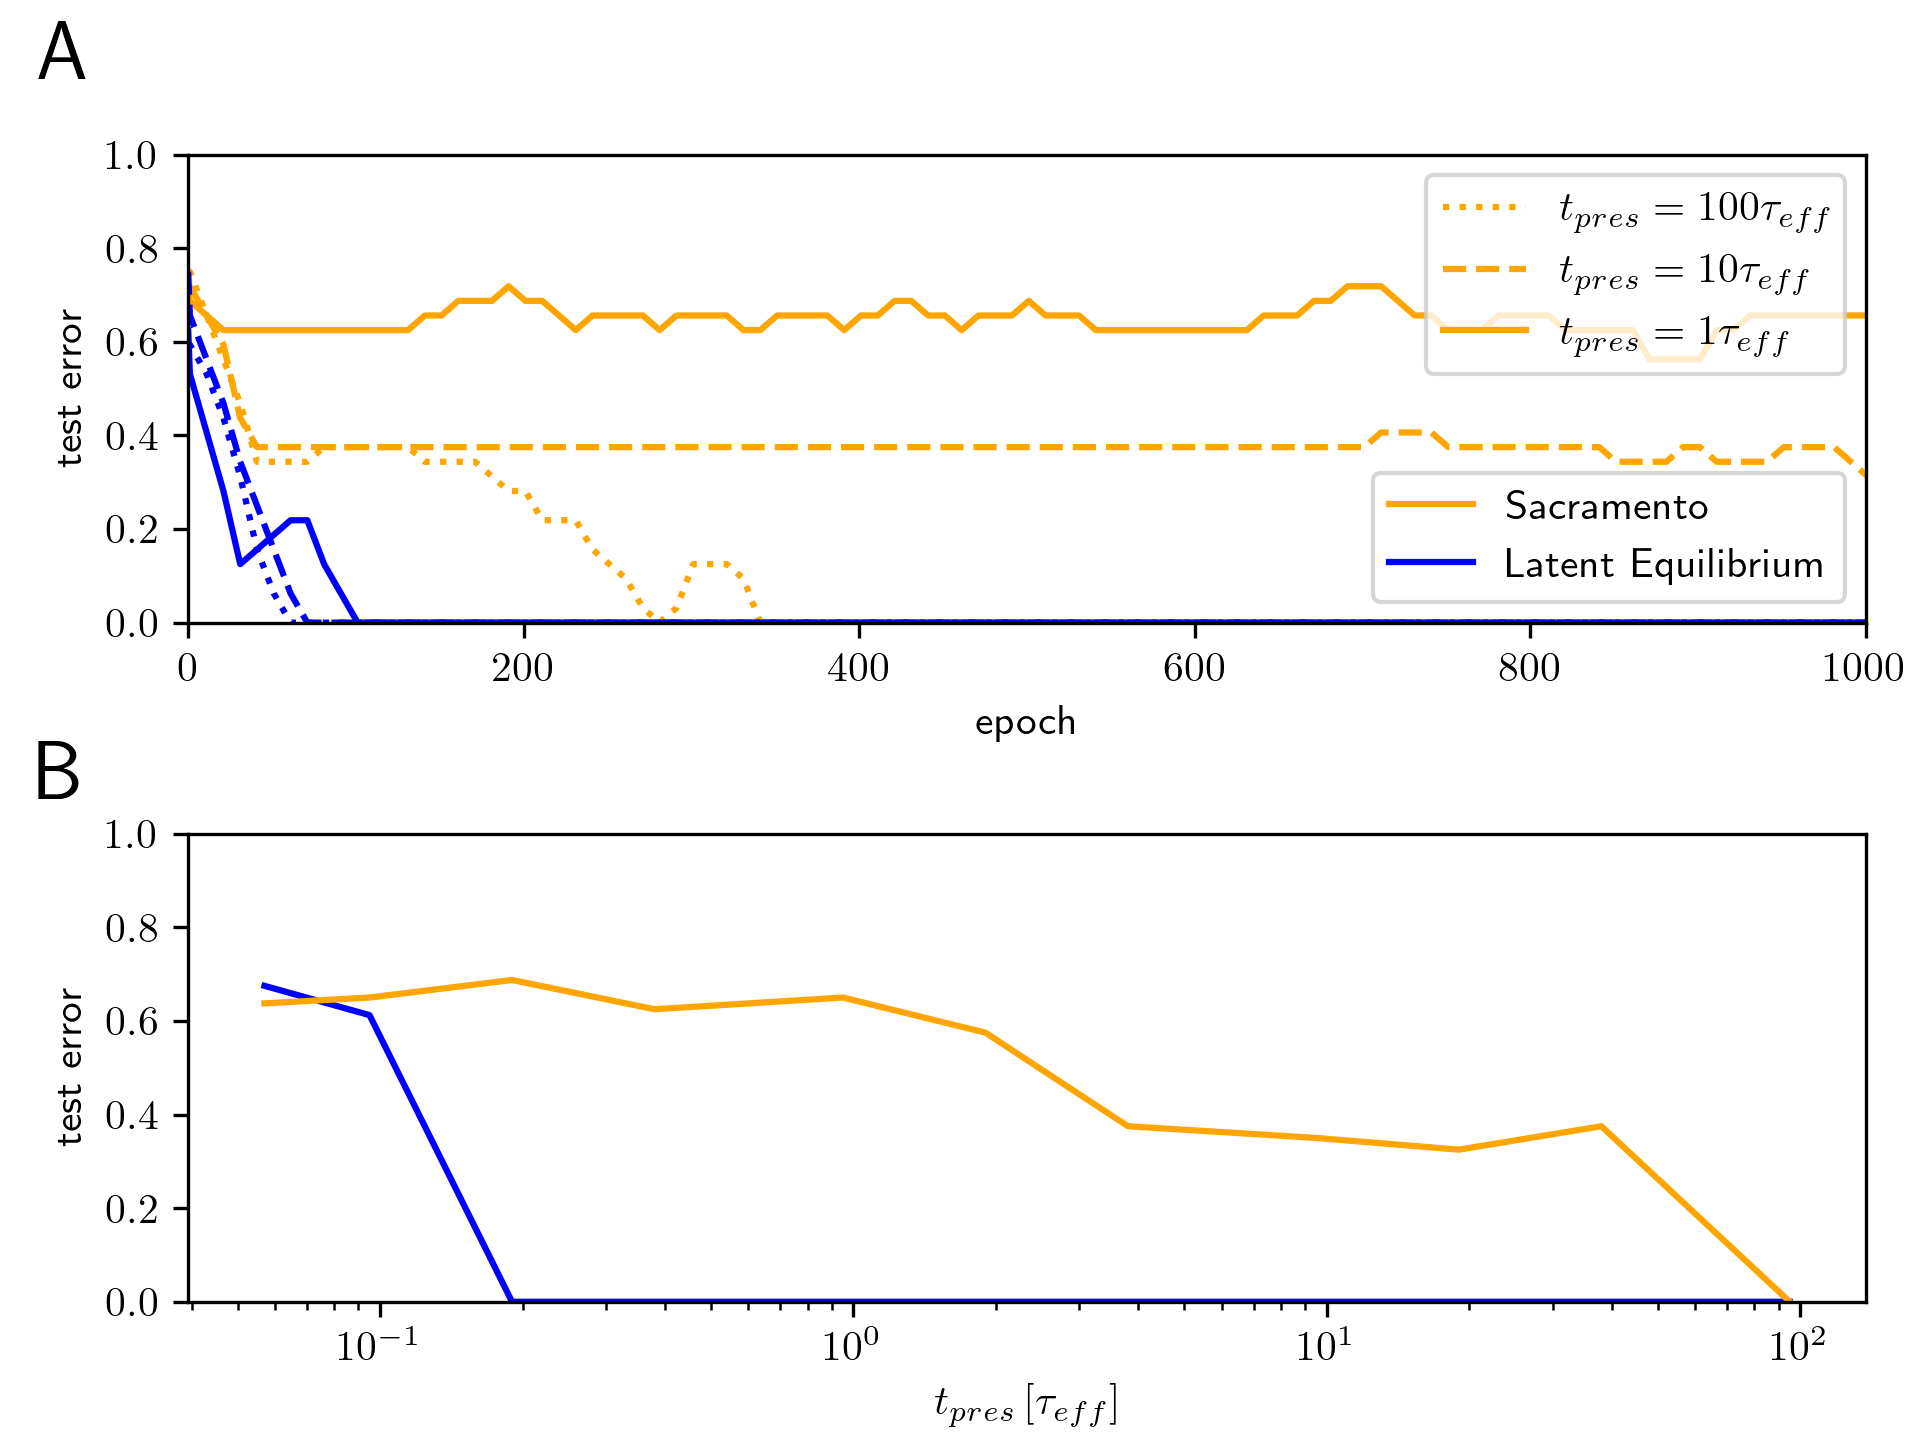
\includegraphics[width=0.9\textwidth]{fig_3_numpy}
    \caption{Replication of Figure \ref{fig-bars-le-snest} using a re-implementation of the \cite{Haider2021} code in
        python. Resulting performance matches the original results exactly, proving that my replication can serve as a
        baseline for comparing the NEST implementation}
    \label{fig-bars-le-numpy}
\end{figure}


\begin{figure}
    \centering
    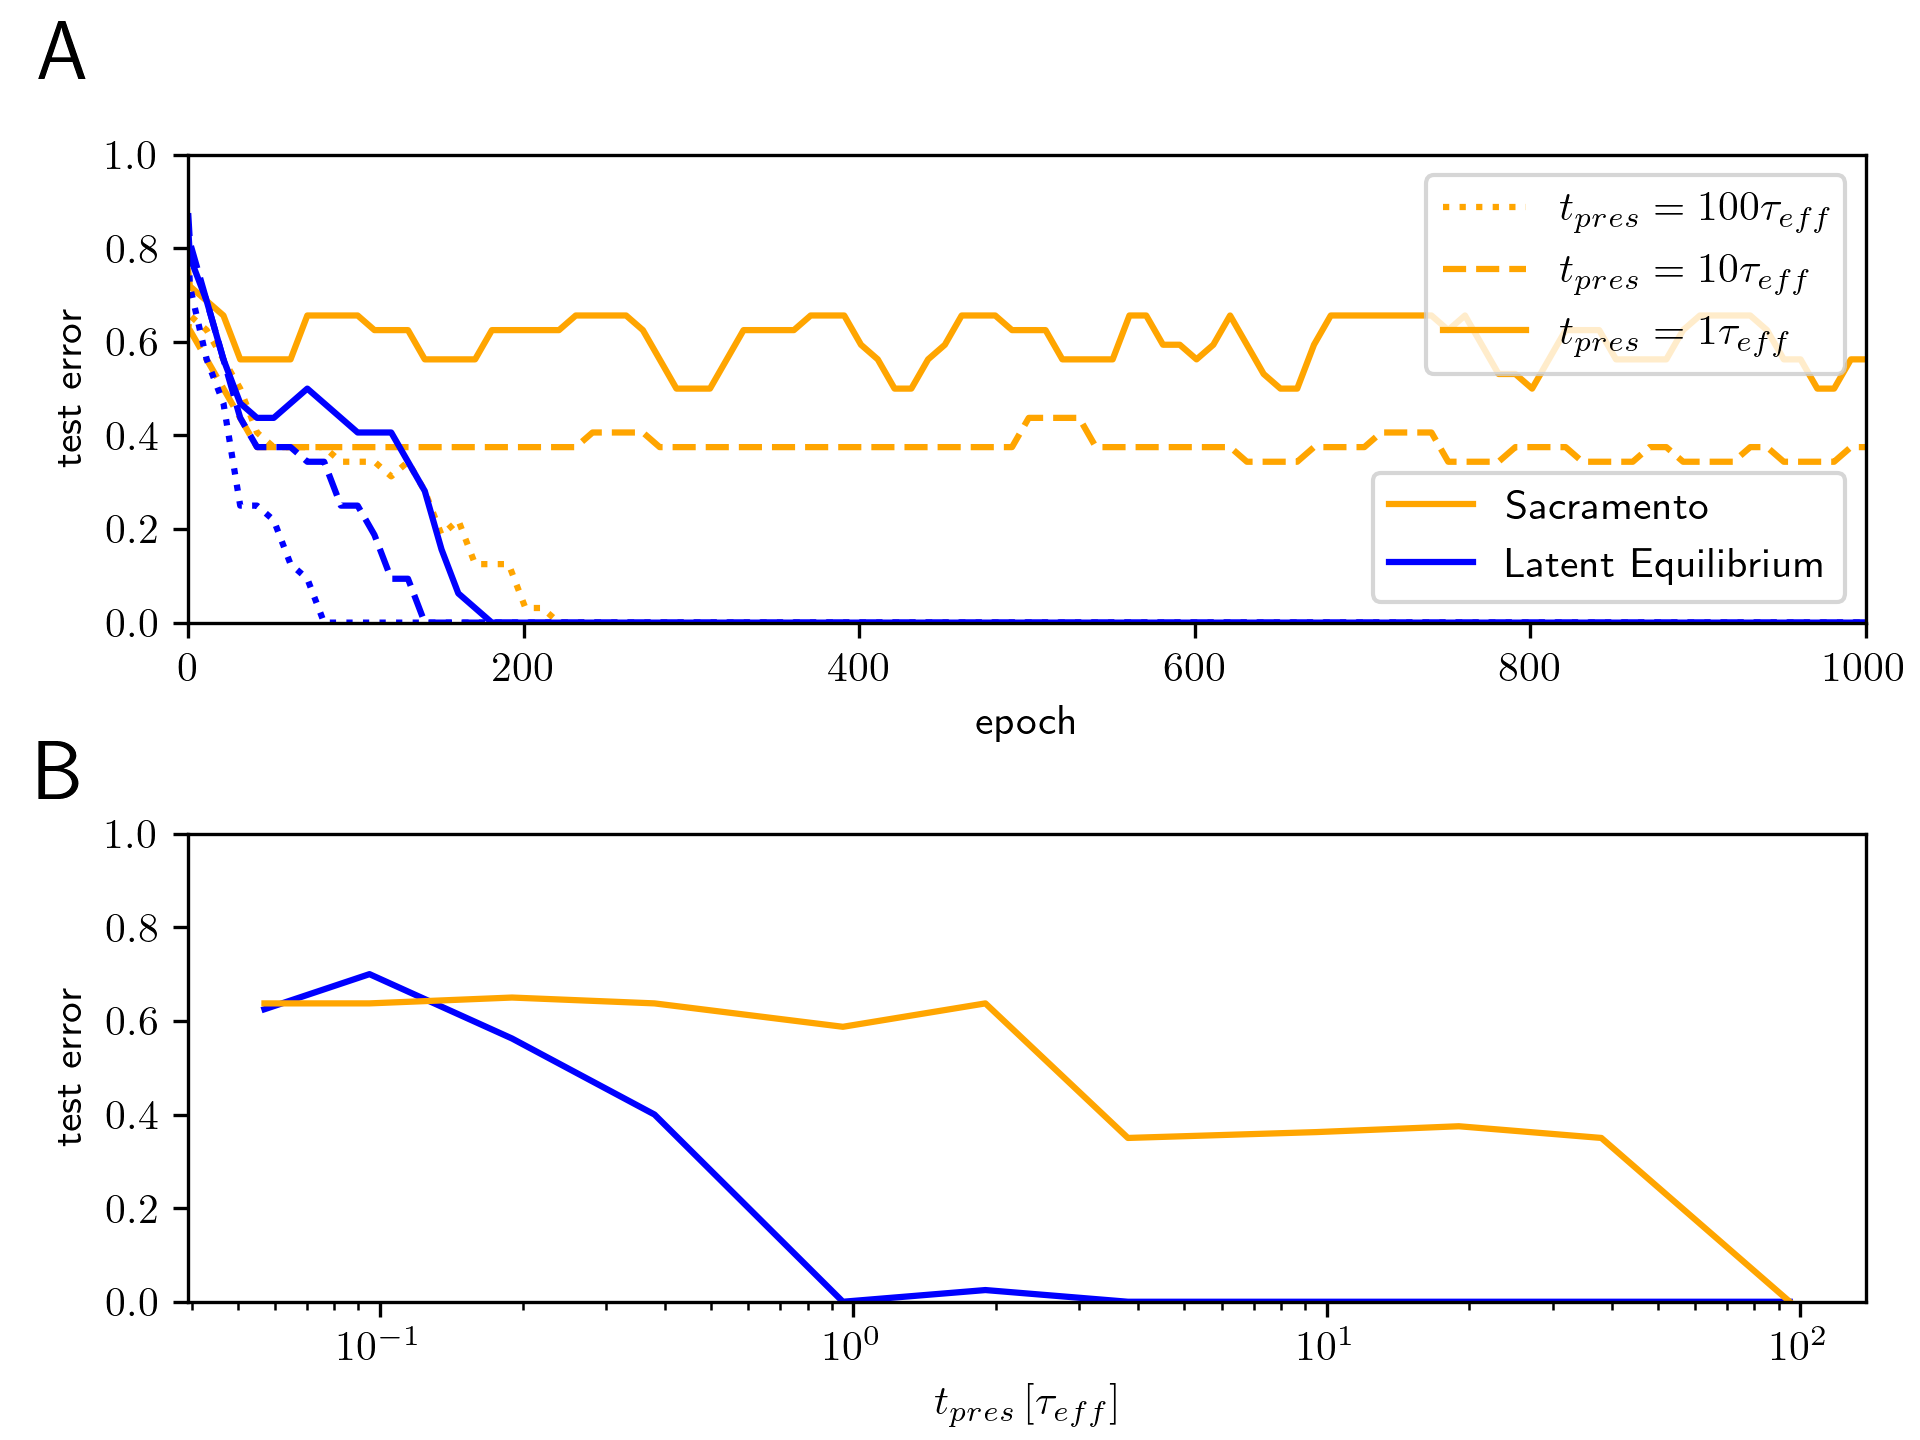
\includegraphics[width=0.9\textwidth]{fig_3_rnest}
    \caption{Replication of Figure \ref{fig-bars-le-snest} using networks of rate neurons in the NEST simulator.}
    \label{fig-bars-le-rnest}
\end{figure}


